\documentclass[11pt, twocolumn]{article}

\usepackage[T2A]{fontenc}
\usepackage[utf8]{inputenc}
\usepackage[english,russian]{babel}

\usepackage[
a4paper,
top=2.5cm,bottom=2.5cm,
left=1.75cm,right=1.75cm,
columnsep=0.5cm
]{geometry}

\usepackage{tempora}
\usepackage{newtxmath}

\usepackage{setspace}
\singlespacing
\usepackage{microtype}
\setlength{\parindent}{1cm}
\setlength{\parskip}{0pt}
\usepackage{indentfirst}
\raggedbottom

\DeclareMathSizes{11}{11}{7}{5}

\usepackage{graphicx}
\usepackage[font={small,bf},labelsep=period]{caption}
\addto\captionsrussian{\renewcommand\figurename{Рис.}}
\addto\captionsrussian{\renewcommand\tablename{Таблица}}

\usepackage{stfloats} 

\usepackage{cuted} 

\usepackage{cite}

\usepackage{titlesec}
\titleformat{\section}
{\bfseries\fontsize{11}{11}\selectfont}
{}
{0pt}
{}
\titlespacing*{\section}
{0pt}
{\baselineskip}
{0pt}

\titleformat{\subsection}
{\bfseries\fontsize{11}{11}\selectfont}
{}
{0pt}
{}
\titlespacing*{\subsection}
{0pt}
{\baselineskip}
{0pt}

\newcommand{\udc}[1]{\noindent\textbf{УДК #1}\par\vspace{0.5em}
}
\newcommand{\ruTitle}[1]{\noindent{\bfseries\fontsize{14}{15}\selectfont #1}\par\vspace{0.75em}
}
\newcommand{\enTitle}[1]{\noindent{\bfseries\fontsize{14}{15}\selectfont #1}\par\vspace{0.75em}
}
\newcommand{\ruAuthors}[1]{\noindent{\bfseries #1}\par
}
\newcommand{\enAuthors}[1]{\noindent{\bfseries #1}\par
}
\newcommand{\ruAffiliations}[1]{\noindent{\itshape\small #1}\par\vspace{0.5em}
}
\newcommand{\enAffiliations}[1]{\noindent{\itshape\small #1}\par\vspace{0.5em}
}
\newcommand{\AuthorEmail}[1]{\noindent{\small #1}\par\vspace{0.75em}
}
\newcommand{\ruAbstract}[1]{\noindent\textbf{Резюме}\par
	\noindent #1\par\vspace{0.75em}
}
\newcommand{\enAbstract}[1]{\noindent\textbf{Abstract}\par
	\noindent #1\par\vspace{0.75em}
}
\newcommand{\ruKeywords}[1]{\noindent\textbf{Ключевые слова}\par
	\noindent #1\par\vspace{0.75em}
}
\newcommand{\enKeywords}[1]{\noindent\textbf{Keywords}\par
	\noindent #1\par\vspace{0.75em}
}
\newcommand{\ForCitation}[1]{\noindent\textbf{Для цитирования}\par
	\noindent #1\par\vspace{0.75em}
}
\newcommand{\ArticleInfo}[1]{\noindent\textbf{Информация о статье}\par
	\noindent #1\par\vspace{0.75em}
}
\newcommand{\Acknowledgements}[1]{\noindent\textbf{Благодарность}\par
	\noindent #1\par\vspace{0.75em}
}
\makeatletter
\renewenvironment{thebibliography}[1]
{\list{\@biblabel{\@arabic\c@enumiv}}{\settowidth\labelwidth{\@biblabel{#1}}\leftmargin\labelwidth
		\advance\leftmargin\labelsep
		\@openbib@code
		\usecounter{enumiv}\let\p@enumiv\@empty
		\renewcommand\theenumiv{\@arabic\c@enumiv}}\sloppy
	\clubpenalty4000
	\widowpenalty4000
	\sfcode`\.\@m}
{\def\@noitemerr
	{\@latex@warning{Empty `thebibliography' environment}}\endlist}
\makeatother

\newcommand{\bicaption}[2]{\caption{#1}\vspace{-0.7em} {\captionsetup{labelformat=empty}
		\caption*{\textbf{Fig.~\thefigure.} #2}}
} \usepackage{comment}
\usepackage{color}
\usepackage{placeins}
\usepackage{graphicx} 
\begin{document}
	
\raggedbottom
\setlength{\parskip}{0pt}
\twocolumn[{
	\begin{minipage}{\textwidth}
		\udc{004.9}

\ruTitle{ОЦИФРОВКА ХИМИЧЕСКИХ КНИГ С ИСПОЛЬЗОВАНИЕМ МАШИННОГО ЗРЕНИЯ}

\ruAuthors{Алакшин М.\,С.$^{1,2}$, Рыбак А.\,В.$^{1,2}$, Ткачёв Д.\,А.$^{1,2}$, Трофимов И.\,Л.$^{2,3}$}

\ruAffiliations{	
	$^{1}$~Федеральное государственное бюджетное образовательное учреждение высшего образования «Иркутский государственный университет»\\
	$^{2}$~Федеральный исследовательский центр «Иркутский институт химии им.\ А.\,Е.\ Фаворского Сибирского отделения Российской академии наук», г.~Иркутск\\
	$^{3}$~Государственная публичная научно-техническая библиотека Сибирского отделения Российской академии наук, г.~Новосибирск	
}



\ruAbstract{В статье рассматривается трансформация роли современных библиотек в условиях цифровой неопределенности и стремительного развития технологий искусственного интеллекта. ...
}

\ruKeywords{искусственный интеллект, цифровая неопределенность, информационный шум, генеративные нейронные сети, интеллектуальная поисковая система, Retrieval Augmented Generation, семантический поиск, верификация, научное наследие, большие языковые модели
}

\enTitle{DIGITIZATION OF CHEMISTRY BOOKS USING MACHINE VISION}

\enAuthors{Alakshin M.\,S.$^{1,2}$, Rybak A.\,V.$^{1,2}$, Tkachev D.\,A.$^{1,2}$, Trofimov I.\,L.$^{2,3}$}

\enAffiliations{ 
	$^{1}$~Federal State Budgetary Educational Institution of Higher Education "Irkutsk State University"\\ 
	$^{2}$~Federal Research Center "Irkutsk Institute of Chemistry named after A.\,E.\ Favorsky, Siberian Branch of the Russian Academy of Sciences", ~Irkutsk\\ 
	$^{3}$~State Public Scientific and Technical Library of the Siberian Branch of the Russian Academy of Sciences, ~Novosibirsk
}

\enAbstract{The article examines the transformation of the role of modern libraries in conditions of digital uncertainty and the rapid development of artificial intelligence technologies. ...
}

\enKeywords{artificial intelligence, digital uncertainty, information noise, generative neural networks, intelligent search system, Retrieval Augmented Generation, semantic search, verification, scientific heritage, large language models
} 		\vspace{2em} \end{minipage}
}]

\section*{Введение}
Знания, содержащиеся в химических книгах, монографиях и архивных выпусках журналов, сохраняют высокую научную и практическую ценность: в них зафиксированы методики синтеза, экспериментальные наблюдения, справочные сведения о веществах и их свойствах, а также контекст, необходимый для воспроизводимости результатов. При этом существенная часть такого корпуса литературы до сих пор существует в виде физических изданий или в виде скан-копий, которые удобны для чтения человеком, но плохо приспособлены для автоматизированного анализа и интеграции в современные информационные системы.

На фоне развития информационных технологий и интеллектуального поиска становится актуальной задача извлечения знаний из химических книг с последующей структуризацией и верификацией. Однако на практике оцифровка часто сводится к распознаванию текста (OCR) и формированию <<поискового PDF>>~\cite{refDavletov}, что позволяет выполнять лишь поверхностный текстовый поиск. В химической литературе значимая часть информации представлена не в виде текста, а в виде графических объектов: структурных формул, схем реакций. Если эти элементы не переводятся в машинно-обрабатываемые представления, то большая доля смысла документа остается вне цифрового контура и фактически недоступна для алгоритмов поиска, сопоставления и анализа~\cite{refKuchuganov}.

В данной работе рассматривается подход к комплексной оцифровке химической литературы, ориентированный не только на извлечение текстового слоя, но и на распознавание и структурирование графической химической информации, что позволяет разработать систему интеллектуального поиска по книгам .  

\section{Машинное зрения и проблемы с извлечением данных из сканированных книг}
Машинное зрение (Computer Vision, CV) представляет собой область искусственного интеллекта, изучающую методы автоматического анализа изображений и видео с целью извлечения из них семантически значимой информации~\cite{refRakov}. В работе~\cite{refRublevsky} машинное зрение выделяется как внешних кольцо в общей классификации искусственного интеллекта (см. рис.~\ref{fig:classifications_ai}).
\begin{figure*}[hbtp]
	\centering
	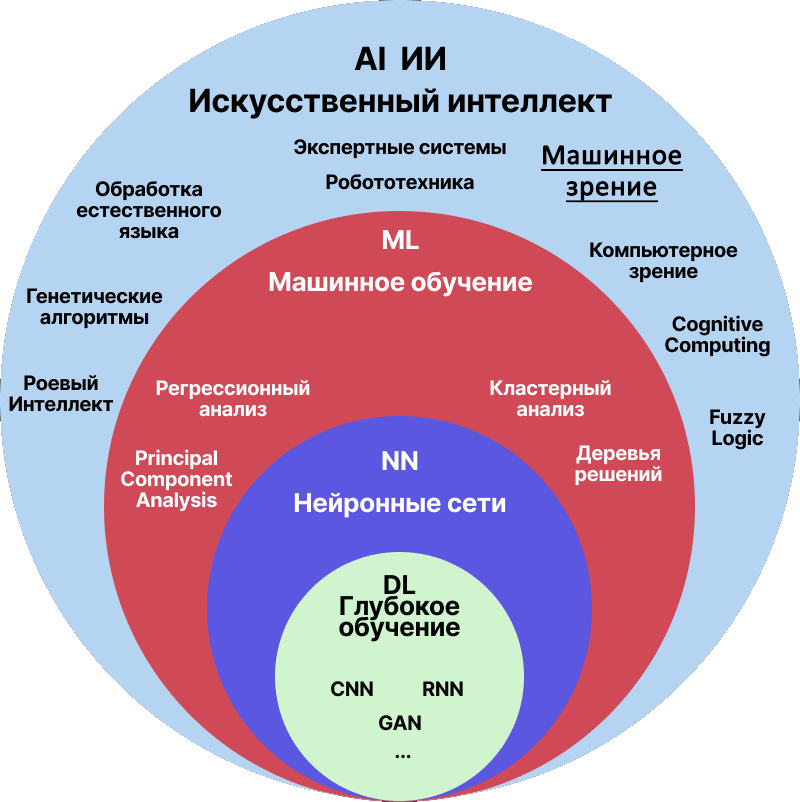
\includegraphics[width=0.5\linewidth]{img/classifications_ai.png}
	\bicaption
	{Классификация искусственного интеллекта}
	{Classification of artificial intelligence}
	\label{fig:classifications_ai}
\end{figure*}
Практическая необходимость применения методов компьютерного зрения в рамках данной работы обусловлена тем, что автоматизация обработки документов требует не только распознавания текста, но и предварительного анализа изображения документа. Как показано в работе А.~Р.~Давлетова, современные OCR-системы решают задачи предварительной обработки изображения, обнаружения текстовых областей, анализа компоновки страницы и последующего распознавания символов и слов~\cite{refDavletov}. Такой подход позволяет преобразовывать сканированные документы, PDF-файлы и изображения, полученные при сканировании, в машиночитаемый текст, пригодный для поиска, редактирования и дальнейшего извлечения данных~\cite{refDavletov}.

По сравнению с ручной обработкой автоматизированный подход сокращает время ввода данных, снижает влияние человеческого фактора, уменьшает количество ошибок и упрощает поиск и доступ к информации~\cite{refDavletov}. Кроме того, в рассматриваемой статье отмечается, что применение методов машинного обучения совместно с OCR позволяет не только конвертировать изображение в текст, но и извлекать из него полезные данные, а в практических сценариях такие решения демонстрируют высокую точность и значительный уровень автоматизации документооборота~\cite{refDavletov}.

 
\section{Сегментация страницы}
Для распознавания документов критично учитывать регулярную структуру страницы и взаимное расположение блоков, поскольку страница научного документа представляет собой не просто непрерывное изображение текста, а композицию из различных смысловых областей: заголовков, основного текста, подписей к рисункам, таблиц, формул, схем, иллюстраций и служебных элементов~\cite{refLayoutLM}.

При этом качество исходного скана также существенно влияет на надежность распознавания: шум, перекос, неравномерная засветка и другие дефекты заметно ухудшают последующие этапы OCR и анализа структуры документа~\cite{refSmith}.

Эта задача относится к направлению анализа изображений документов и играет роль промежуточного звена между общими методами машинного зрения и прикладными системами OCR. Если этап сегментации пропускается или выполняется неточно, то OCR-система может воспринимать графические объекты как текст, объединять соседние колонки, терять подписи к рисункам, ошибочно включать части формул в текстовый поток или, наоборот, игнорировать важные текстовые фрагменты. Для химической литературы данная проблема особенно существенна, поскольку на одной странице часто одновременно присутствуют обычный текст, структурные химические формулы, схемы реакций, таблицы и обозначения, различающиеся как по визуальной форме, так и по способу дальнейшей обработки.

С практической точки зрения сегментация страницы позволяет перейти от обработки документа как единого изображения к обработке набора специализированных областей. После выделения таких областей (см. рис.~\ref{fig:segment}) к каждой из них может быть применен собственный алгоритм: к текстовым блокам --- OCR, к структурным формулам --- методы распознавания химической графики, к таблицам --- алгоритмы восстановления табличной структуры, к рисункам и схемам --- отдельные процедуры анализа изображений. Таким образом, сегментация формирует основу всего конвейера оцифровки: \textit{страница целиком $\rightarrow$ выделение блоков $\rightarrow$ специализированное распознавание $\rightarrow$ структурированное представление знаний}.

\begin{figure*}[t]
	\centering
	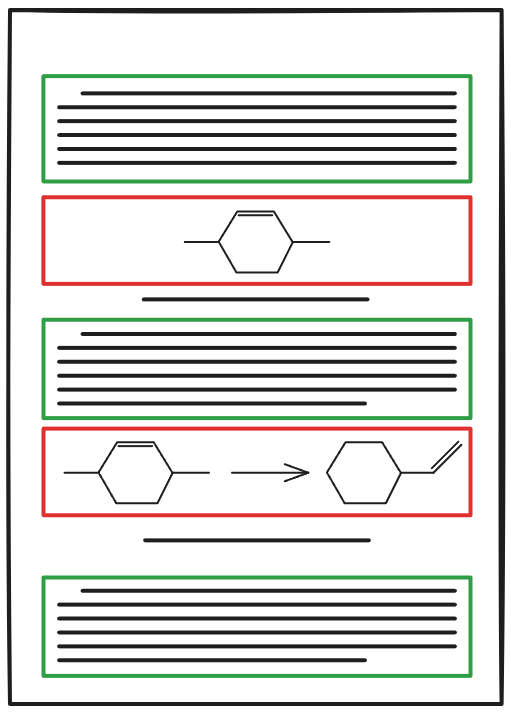
\includegraphics[width=0.3\linewidth]{img/sheme.png}
	\bicaption
	{Схема сегментации}
	{Segmentation scheme}
	\label{fig:segment}
\end{figure*}

Современные подходы к анализу макета документа опираются на методы глубокого обучения, позволяющие автоматически выделять типовые области страницы и учитывать их пространственный контекст. В работе P.~Renton, P.~Chatto и соавторов представлен инструментарий \textit{LayoutParser}, ориентированный на унифицированный анализ структуры документов на основе моделей глубокого обучения, что подтверждает практическую значимость этапа предварительной сегментации для дальнейшего извлечения информации из сложных страниц~\cite{refLayoutParser}. Использование подобных подходов особенно актуально для оцифровки архивных и сканированных книг, где вариативность верстки, качество печати и наличие графических элементов делают задачу прямого распознавания без предварительного структурного анализа существенно менее надежной. 
\section{Предобработка изображения}
Большинство архивных химических книг и сканированных материалов характеризуются неоднородным качеством. В работе~\cite{refAkhil} выделялись следующие проблемы качества сканированных книг:
\begin{itemize}
	\item Низкое разрешение / размытость (рис.~\ref{fig:poor_quality} a)
	\item Шум, зернистость, артефакты сжатия (рис.~\ref{fig:poor_quality} b)
	\item Неравномерная засветлённость / тени (рис.~\ref{fig:poor_quality} c)
	\item Ориентация страницы с малым поворотом (рис.~\ref{fig:poor_quality} d)
\end{itemize}

\begin{figure*}[hbtp]
	\centering
	\begin{tabular}{cc}
		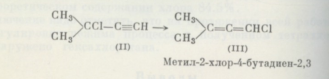
\includegraphics[width=0.25\linewidth]{img/blur.png} & 
		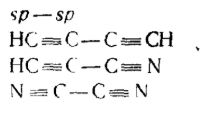
\includegraphics[width=0.25\linewidth]{img/grain.png} \\
		a$)$ & b$)$\\
		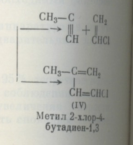
\includegraphics[width=0.25\linewidth]{img/flashing.png} & 
		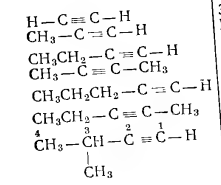
\includegraphics[width=0.25\linewidth]{img/orientation.png}\\
		c$)$ & d$)$		
	\end{tabular}
	\bicaption
	{Пример плохого качества сканированных книг
		a) Размытость; b) Шум; c) Неравномерная засветлённость; d) Ориентация страницы с малым поворотом.
	}
	{An example of poor quality scanned books 
		a) Blur; b) Noise; c) Uneven illumination; d) Page orientation with low rotation.	
	}
	\label{fig:poor_quality}
\end{figure*}

Эти факторы напрямую влияют на точность распознания как и графических формул и реакций так и текста. Поэтому перед обработкой самой OCR необходимо сделать пред обработку и нормализацию изображения. 



 
\section{Проблемы с преобразование химических реакций и молекул в машиначитабельный вид}
Химические формулы и схемы реакций существенно сложнее для автоматической обработки, чем обычный текст, поскольку их естественное представление является не линейной последовательностью символов, а графовой структурой. В молекулярном графе вершины соответствуют атомам, а рёбра — химическим связям; реакция, в свою очередь, может рассматриваться как преобразование одного множества молекулярных графов в другое. Поэтому химическая запись несёт смысл не только через набор символов, но и через топологию, тип связей, ароматичность, заряды, стереохимию и пространственные отношения между фрагментами структуры. Именно это отличает задачу распознавания формул от классического OCR: если для текста ключевой является последовательность символов, то для химической формулы необходимо восстановить структуру графа и затем представить её в форме, пригодной для хранения, поиска и последующего анализа \cite{refTrinajstic,refWarr}.

Дополнительную сложность создаёт то, что в химической литературе используются по меньшей мере две распространённые графические нотации записи молекул: подробная (развёрнутая) и скелетная (см. рис.~\ref{fig:comparison_notations}). В подробной записи явно показываются атомы и значительная часть связей, что облегчает интерпретацию человеком, но увеличивает визуальную насыщенность изображения. В скелетной нотации, напротив, большинство атомов углерода и связанные с ними атомы водорода опускаются, а углеродный каркас кодируется линиями, вершины и концы которых интерпретируются как атомы углерода; гетероатомы, кратные связи, заряды и функциональные группы отображаются явно. Именно скелетная запись наиболее типична для органической химии и научных публикаций, однако она значительно усложняет автоматическое распознавание, так как часть информации в ней задаётся по соглашению, а не прописывается явно. В результате алгоритм должен не просто “увидеть линии”, но восстановить скрытые атомы, валентности и химически допустимую структуру \cite{refWarr}.

\begin{figure*}[hbtp]
	\centering
	\begin{tabular}{cc}
		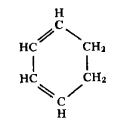
\includegraphics[width=0.25\linewidth]{img/detailed_form.png} & 
		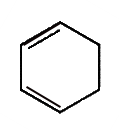
\includegraphics[width=0.25\linewidth]{img/skeletal_form.png} \\
		a$)$ & b$)$	
	\end{tabular}
	\bicaption
	{Пример разных нотаций
		a) подробная; b) скелетная.
	}
	{Example of different notations 
		a) detailed; b) skeletal.	
	}
	\label{fig:comparison_notations}
\end{figure*}

После распознавания графическое изображение молекулы должно быть переведено в машинно-обрабатываемый формат. В современной хемоинформатике для этого используются несколько основных способов представления структур. К числу наиболее распространённых относятся SMILES (Simplified Molecular Input Line Entry System), InChI (International Chemical Identifier), файловые форматы Molfile и SDF, XML-ориентированный CML (Chemical Markup Language), а для реакций — RXNfile, RDF, а также строковые языки наподобие SMIRKS для описания реакционных преобразований. Эти форматы различаются по назначению: одни удобны для компактной линейной записи и поиска, другие — для хранения полной структурной информации, координат, метаданных и реакционных схем. Обзор таких представлений и их роли в химической информатике приведён в работах по компьютерному представлению химических структур и форматам химических данных \cite{refWarr,refDalby,refInChI}.

В данной работе в качестве основного текстового представления структуры выбран формат SMILES, предложенный как компактный язык линейной записи молекул \cite{refWeininger1,refWeininger2}. Его выбор обусловлен несколькими причинами. Во-первых, SMILES является кратким и человекочитаемым: одна молекула кодируется строкой, удобной для хранения в базах данных, индексации, поиска и передачи между программными компонентами. Во-вторых, SMILES широко поддерживается в современных библиотеках и инструментах хемоинформатики, что облегчает интеграцию распознанных структур в конвейер обработки, верификации и поиска. В-третьих, SMILES особенно удобен в задачах, где химическая информация должна быть включена в текстовый или гибридный контур обработки — например, при индексировании документов, построении RAG-систем, текстовом сравнении структур или использовании языковых моделей. В отличие от графического изображения, строка SMILES может быть быстро сопоставлена, нормализована, проверена на корректность и преобразована обратно в молекулярный граф, что делает её практическим компромиссом между компактностью, выразительностью и вычислительной удобностью \cite{refWeininger1,refWarr}.

При этом важным свойством SMILES является неоднозначность представления (см. рис.~\ref{fig:ambiguity_smileys}): одна и та же молекула может быть записана несколькими различными, но эквивалентными строками. Это связано с тем, что линейная запись строится на основе обхода графа, а один и тот же граф допускает разные порядки обхода, разные точки старта, разные способы нумерации циклов, а также различные варианты явного или неявного задания некоторых структурных особенностей. Например, одна и та же структура может быть записана через разные эквивалентные последовательности ветвлений или с использованием разных соглашений для ароматических фрагментов. В задачах хранения и поиска это создаёт проблему: если использовать произвольный SMILES, то идентичные молекулы могут быть представлены разными строками, что затрудняет дедупликацию, построение индексов и сопоставление результатов распознавания \cite{refWeininger2}.

\begin{figure*}[hbtp]
	\centering
	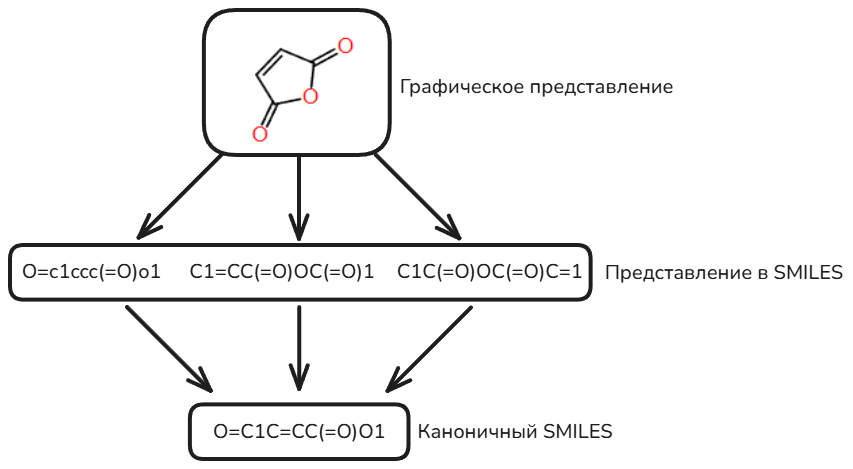
\includegraphics[width=0.75\linewidth]{img/canon_smailes.png}
	\bicaption
	{пример неоднозначного представление форму}
	{example of ambiguous form representation}
	\label{fig:ambiguity_smileys}
\end{figure*}

Для устранения этой неоднозначности используется канонический SMILES, то есть строковое представление, которое строится по детерминированному алгоритму канонизации и назначает данной структуре единственную <<стандартную>> форму записи в рамках конкретной программной системы. Идея канонизации состоит в том, чтобы сначала определить уникальный порядок атомов на основе свойств графа, а затем сгенерировать строку по фиксированным правилам обхода. Это позволяет переводить множество эквивалентных SMILES-представлений одной и той же молекулы к одной нормализованной форме. Однако важно учитывать, что канонический SMILES не является абсолютно универсальным мировым стандартом: разные программные пакеты могут использовать разные алгоритмы канонизации, поэтому канонические строки, полученные, например, в двух различных хемоинформатических библиотеках, могут отличаться при сохранении химической эквивалентности. Тем не менее в рамках одного конвейера обработки канонический SMILES является чрезвычайно полезным инструментом, поскольку обеспечивает нормализацию результатов распознавания, устойчивое сравнение структур и корректную интеграцию извлечённых данных в базы знаний и поисковые индексы \cite{refWeininger2,refOBoyleCanonical,refInChI}. Таким образом, выбор SMILES в сочетании с последующей канонизацией представляет собой практически оправданное решение для задач оцифровки и структурирования химической литературы.

 
Поэтому задача комплексной оцифровки требует:
\begin{enumerate}
	\item сегментации страницы на логические блоки
	\item предварительной визуальной нормализации изображения
	\item специализированных методов извлечения
	\item сама обработка 
\end{enumerate}
  \section{Программное обеспечения для обработки страниц химических книг}
В рамках настоящей работы, опираясь на результаты анализа предметной области и выявленные ограничения существующих подходов, было разработано программное обеспечение для оцифровки страниц химических книг. Функциональная логика системы и основные этапы обработки данных представлены на UML-диаграмме активностей~\cite{refUML} (рис.~\ref{fig:bisnes}).

\begin{figure*}[t]
	\centering
	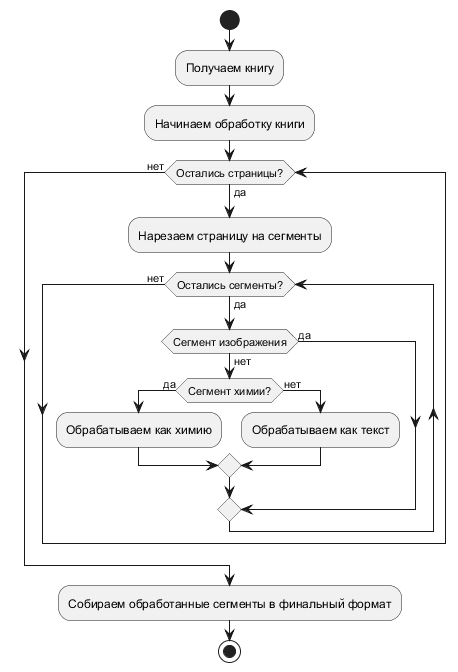
\includegraphics[width=0.35\linewidth]{img/chemistry_books_bisnes.png}
	\bicaption
	{UML-диаграмма активностей программы по обработке страниц книг по химии}
	{UML activity diagram of a program for processing pages of chemistry books}
	\label{fig:bisnes}
\end{figure*}

Программный комплекс реализован на языке Python, что объясняется его практической востребованностью в задачах обработки изображений и разработки интеллектуальных систем анализа документов. При проектировании использовались паттерны объектно-ориентированного проектирования~\cite{refGoF}, позволившие структурировать приложение и упростить его дальнейшее расширение. Для обеспечения единообразия и читаемости исходного кода соблюдались рекомендации Python Enhancement Proposals, в частности стандарты оформления кода PEP~8~\cite{refPEP8}. 
\section{Обработка молекул}
На основе представления молекул в формате SMILES было разработано программное обеспечение для распознавания химических структур по изображениям. Для решения данной задачи применяются методы OCSR (Optical Chemical Structure Recognition — оптическое распознавание химических структур)~\cite{refWikiOCSR}. Следует отметить, что OCSR представляет собой не отдельный тип модели, а прикладную задачу, для решения которой используются методы компьютерного зрения и глубокого обучения. В контексте классификации искусственного интеллекта такие методы относятся к области глубокого обучения, представленной на рис.~\ref{fig:classifications_ai} как наиболее внутренний уровень иерархии.

В качестве основы для анализа были рассмотрены три модели, представляющие различные подходы к задаче OCSR:

\begin{enumerate}
	\item \textbf{MolScribe.}  
	MolScribe представляет собой структурно-ориентированный подход к распознаванию химических изображений. Ключевая идея модели заключается в том, что химическую структуру целесообразно рассматривать не как набор независимых символов или линий, а как молекулярный граф, который затем может быть преобразован в строковое представление. В рамках данного подхода изображение сначала переводится в набор визуальных признаков, после чего на их основе восстанавливается структура молекулы~\cite{refMolScribe}. Таким образом, модель определяет положение атомов, типы связей между ними, наличие ароматичности, зарядов и особенности стереохимии. Благодаря этому MolScribe можно отнести к моделям, ориентированным на восстановление химического графа, а не только на последовательное распознавание элементов изображения.
	
	\item \textbf{DECIMER (Deep Learning for Chemical Image Recognition).}  
	DECIMER представляет собой модель OCSR, основанную на методах глубокого обучения и обученную на больших объёмах синтетически сгенерированных данных~\cite{refDECIMER}. Архитектурно данный подход ориентирован на преобразование изображения химической структуры в строковое представление молекулы. В основе модели лежит схема, в которой сначала из изображения извлекаются визуальные признаки, а затем они используются для генерации последовательности токенов, описывающих химическую структуру. В качестве текстового представления в DECIMER применяется SELFIES, что позволяет повысить устойчивость генерации по сравнению с непосредственным предсказанием SMILES~\cite{refDECIMERJournal}. Существенным достоинством DECIMER является высокая точность распознавания на больших наборах данных, однако по сравнению с графо-ориентированными подходами модель в меньшей степени отражает молекулу именно как графовую структуру, поскольку её основной выход формируется в виде последовательности символов~\cite{refDECIMERJournal}.
	
	\item \textbf{Qwen3-VL.}  
	Qwen3-VL представляет собой мультимодальную vision-language модель, способную анализировать графическую информацию и формировать текстовое описание содержимого изображения. В контексте задачи OCSR такая модель может рассматриваться как универсальный инструмент визуально-текстового преобразования, потенциально пригодный для интерпретации изображений химических структур. В отличие от специализированных моделей, таких как MolScribe и DECIMER, Qwen3-VL не разрабатывалась исключительно для задач химического распознавания, однако её мультимодальная архитектура позволяет использовать её в качестве сравнительного или вспомогательного подхода при анализе химических изображений~\cite{refQwen3VL}.
\end{enumerate}

Для применения моделей MolScribe и DECIMER в работе использовались их встроенные механизмы обработки изображений химических структур. В случае Qwen3-VL взаимодействие с моделью осуществлялось программно через API с использованием системного промпта и набора демонстрационных примеров. Такой подход соответствует парадигме few-shot in-context learning, при которой модель адаптируется к требуемому формату ответа на основе контекста запроса без дополнительного дообучения параметров модели.

Концептуально использование few-shot in-context learning в молекулярных задачах согласуется с результатами работы C.~Fifty, J.~Leskovec и S.~Thrun, где предложен алгоритм CAMP для few-shot предсказания молекулярных свойств~\cite{refCAMP}. В данной статье показано, что модель может выполнять предсказание на основе контекста из пар «объект--метка» за один проход, без этапа fine-tuning, и при малом числе примеров превосходит ряд классических meta-learning-подходов~\cite{refCAMP}. Хотя работа~\cite{refCAMP} посвящена не распознаванию химических структур по изображениям, а задаче предсказания молекулярных свойств, она подтверждает применимость самой идеи in-context learning в химических задачах при ограниченном числе демонстраций. Поэтому в настоящей работе данный принцип используется как методологическое основание для применения Qwen3-VL в задаче распознавания химических формул по изображениям: модели предоставляется системная инструкция и несколько примеров соответствия между изображением структуры и требуемым текстовым представлением.
 
\section{Предобработка изображений}
 
Было взято набор изображений молекул из сканированный книг в центральная научная библиотека Иркутского научного центра Сибирского отделения Российской академии наук было собранно 20 молекул 10 из которых в скелетной нотации, а 10 в подробная нотации.       


\begin{strip}
	\begin{center}
		\textbf{Список литературы}
	\end{center}
	\begin{thebibliography}{99}
		\small
		\bibitem{refKuchuganov}
Кучуганов, А. В. Методология семантического анализа и поиска графической информации : автореферат диссертации на соискание ученой степени доктора технических наук : специальность 05.13.01 «Системный анализ, управление и обработка информации (в промышленности)» / А. В. Кучуганов. – Ижевск, 2018. – Текст : непосредственный.
\bibitem{refDavletov}
Давлетов, А. Р. Современные методы машинного обучения и технология OCR для автоматизации обработки документов / А. Р. Давлетов. – Текст : электронный // Вестник науки. – 2023. – № 10 (67). – URL: https://cyberleninka.ru/article/n/sovremennye-metody-mashinnogo-obucheniya-i-tehnologiya-ocr-dlya-avtomatizatsii-obrabotki-dokumentov (дата обращения: 22.05.2026).
\bibitem{refRakov}
Раков, Н. С. Машинное зрение / Н. С. Раков, С. В. Пальмов. – Текст : электронный // Форум молодых ученых. – 2018. – № 4 (20). – URL: https://cyberleninka.ru/article/n/mashinnoe-zrenie (дата обращения: 22.05.2026).
\bibitem{refRublevsky}
Рублевский, Р. Ландшафт основных терминов в области генеративного AI, их взаимосвязь и употребление / Р. Рублевский. – Текст : электронный // Хабр. – 2025. – 25 сент. – URL: https://habr.com/ru/articles/950600/ (дата обращения: 22.05.2026).
\bibitem{refAkhil}
Akhil, S. Overview of Tesseract OCR engine / S. Akhil. – Текст : электронный // ResearchGate. – 2016. – Dec. – URL: https://www.researchgate.net/publication/315834331 (дата обращения: 22.05.2026).
\bibitem{refLayoutParser}
Shen, Z. LayoutParser: A Unified Toolkit for Deep Learning Based Document Image Analysis / Z. Shen [et al.]. – Текст : электронный // arXiv.org. – 2021. – arXiv:2103.15348. – URL: https://arxiv.org/abs/2103.15348 (дата обращения: 22.05.2026).
\bibitem{refLayoutLM}
Xu, Y. LayoutLM: Pre-training of Text and Layout for Document Image Understanding / Y. Xu, M. Li, L. Cui [et al.]. – Текст : электронный // arXiv.org. – 2019. – arXiv:1912.13318. – URL: https://arxiv.org/abs/1912.13318 (дата обращения: 22.05.2026).
\bibitem{refSmith}
Smith, R. An Overview of the Tesseract OCR Engine / R. Smith // Ninth International Conference on Document Analysis and Recognition (ICDAR 2007). – Washington : IEEE Computer Society, 2007. – Vol. 2. – P. 629--633. – DOI: 10.1109/ICDAR.2007.4376991. – URL: https://doi.org/10.1109/ICDAR.2007.4376991 (дата обращения: 22.05.2026).
\bibitem{refTrinajstic}
Trinajstić, N. Chemical Graph Theory / N. Trinajstić. – 2nd ed. – Boca Raton : CRC Press, 1992. – 364 p.

\bibitem{refWarr}
Warr, W. A. Representation of Chemical Structures / W. A. Warr // Wiley Interdisciplinary Reviews: Computational Molecular Science. – 2011. – Vol. 1, no. 4. – P. 557--579. – DOI: 10.1002/wcms.36.

\bibitem{refWeininger1}
Weininger, D. SMILES, a Chemical Language and Information System. 1. Introduction to Methodology and Encoding Rules / D. Weininger // Journal of Chemical Information and Computer Sciences. – 1988. – Vol. 28, no. 1. – P. 31--36. – DOI: 10.1021/ci00057a005.

\bibitem{refWeininger2}
Weininger, D. SMILES. 2. Algorithm for Generation of Unique SMILES Notation / D. Weininger, A. Weininger, J. L. Weininger // Journal of Chemical Information and Computer Sciences. – 1989. – Vol. 29, no. 2. – P. 97--101. – DOI: 10.1021/ci00062a008.

\bibitem{refDalby}
Dalby, A. Description of Several Chemical Structure File Formats Used by Computer Programs Developed at Molecular Design Limited / A. Dalby, J. G. Nourse, W. D. Hounshell [et al.] // Journal of Chemical Information and Computer Sciences. – 1992. – Vol. 32, no. 3. – P. 244--255. – DOI: 10.1021/ci00007a012.

\bibitem{refInChI}
Heller, S. R. InChI, the IUPAC International Chemical Identifier / S. R. Heller, A. McNaught, I. Pletnev [et al.] // Journal of Cheminformatics. – 2015. – Vol. 7. – Art. 23. – DOI: 10.1186/s13321-015-0068-4.

\bibitem{refOBoyleCanonical}
O'Boyle, N. M. Towards a Universal SMILES Representation – A Standard Method to Generate Canonical SMILES Based on the InChI / N. M. O'Boyle // Journal of Cheminformatics. – 2012. – Vol. 4. – Art. 22. – DOI: 10.1186/1758-2946-4-22.

\bibitem{refWikiOCSR}
Optical chemical structure recognition. – Текст : электронный // Wikipedia. – URL: $https://en.wikipedia.org/wiki/Optical_chemical_structure_recognition$ (дата обращения: 22.05.2026).

\bibitem{refUML}
OMG Unified Modeling Language (OMG UML), Version 2.5.1 / Object Management Group. – 2017. – URL: https://www.omg.org/spec/UML/2.5.1/PDF (дата обращения: 22.05.2026).

\bibitem{refMolScribe}
MolScribe: Robust Molecular Structure Recognition with Image-To-Graph Generation / Y. Qian, J. Guo, Z. Tu [et al.]. – Текст : электронный // arXiv.org. – 2022. – arXiv:2205.14311. – URL: https://arxiv.org/pdf/2205.14311 (дата обращения: 22.05.2026).

\bibitem{refDECIMER}
Rajan, K. DECIMER 1.0: deep learning for chemical image recognition using transformers / K. Rajan [et al.]. – Текст : электронный // ResearchGate. – 2021. – Aug. – URL: $https://www.researchgate.net/publication/353957394_DECIMER_10_deep_learning_for_chemical_image_recognition_using_transformers$ (дата обращения: 22.05.2026).

\bibitem{refDECIMERJournal}
Rajan, K. DECIMER 1.0: deep learning for chemical image recognition using transformers / K. Rajan, A. Zielesny, C. Steinbeck. – Текст : электронный // Journal of Cheminformatics. – 2021. – Vol. 13. – DOI: 10.1186/s13321-021-00538-8. – URL: https://doi.org/10.1186/s13321-021-00538-8 (дата обращения: 22.05.2026).

\bibitem{refQwen3VL}
Qwen Team. Qwen3-VL Technical Report / Qwen Team. – Текст : электронный // arXiv.org. – 2025. – arXiv:2511.21631. – URL: https://arxiv.org/abs/2511.21631 (дата обращения: 22.05.2026).

\bibitem{refCAMP}
Fifty, C. In-Context Learning for Few-Shot Molecular Property Prediction / C. Fifty, J. Leskovec, S. Thrun. – Текст : электронный // arXiv.org. – 2023. – arXiv:2310.08863. – URL: https://arxiv.org/abs/2310.08863 (дата обращения: 22.05.2026).

\bibitem{refGoF}
Gamma, E. Design Patterns: Elements of Reusable Object-Oriented Software / E. Gamma, R. Helm, R. Johnson, J. Vlissides. – Reading : Addison-Wesley, 1995. – 395 p. – ISBN 0-201-63361-2. – Текст : непосредственный.

\bibitem{refPEP8}
van Rossum, G. PEP 8 -- Style Guide for Python Code / G. van Rossum, B. Warsaw, A. Coghlan. – Текст : электронный // Python.org. – URL: https://peps.python.org/pep-0008/ (дата обращения: 23.05.2026).
 	\end{thebibliography}

	\begin{center}
		\textbf{References}
	\end{center}
	\begin{thebibliography}{99}
		\small
		\bibitem{refKuchuganov}
Kuchuganov, A. V. Methodology of semantic analysis and search for graphic information: abstract of the dissertation for the degree of Doctor of Technical Sciences: specialty 05.13.01 “System analysis, management and information processing (in industry)” / A. V. Kuchuganov. – Izhevsk, 2018. – Text: direct.
\bibitem{refDavletov}
Davletov, A. R. Modern methods of machine learning and OCR technology for automating document processing / A. R. Davletov. – Text: electronic // Bulletin of Science. – 2023. – No. 10 (67). – URL: https://cyberleninka.ru/article/n/sovremennye-metody-mashinnogo-obucheniya-i-tehnologiya-ocr-dlya-avtomatizatsii-obrabotki-dokumentov (date of access: 05/22/2026).
\bibitem{refRakov}
Rakov, N. S. Machine vision / N. S. Rakov, S. V. Palmov. – Text: electronic // Forum of young scientists. – 2018. – No. 4 (20). – URL: https://cyberleninka.ru/article/n/mashinnoe-zrenie (date of access: 05/22/2026).
\bibitem{refRublevsky}
Rublevsky, R. Landscape of basic terms in the field of generative AI, their relationship and use / R. Rublevsky. – Text: electronic // Habr. – 2025. – September 25 – URL: https://habr.com/ru/articles/950600/ (access date: 05/22/2026).
\bibitem{refAkhil}
Akhil, S. Overview of Tesseract OCR engine / S. Akhil. – Text: electronic // ResearchGate. – 2016. – Dec. – URL: https://www.researchgate.net/publication/315834331 (access date: 05/22/2026).
\bibitem{refLayoutParser}
Shen, Z. LayoutParser: A Unified Toolkit for Deep Learning Based Document Image Analysis / Z. Shen [et al.]. – Text: electronic // arXiv.org. – 2021. – arXiv:2103.15348. – URL: https://arxiv.org/abs/2103.15348 (access date: 05/22/2026).
\bibitem{refLayoutLM}
Xu, Y. LayoutLM: Pre-training of Text and Layout for Document Image Understanding / Y. Xu, M. Li, L. Cui [et al.]. – Text: electronic // arXiv.org. – 2019. – arXiv:1912.13318. – URL: https://arxiv.org/abs/1912.13318 (access date: 05/22/2026).
\bibitem{refSmith}
Smith, R. An Overview of the Tesseract OCR Engine / R. Smith // Ninth International Conference on Document Analysis and Recognition (ICDAR 2007). – Washington: IEEE Computer Society, 2007. – Vol. 2. – P. 629--633. – DOI: 10.1109/ICDAR.2007.4376991. – URL: https://doi.org/10.1109/ICDAR.2007.4376991 (access date: 05.22.2026).
\bibitem{refTrinajstic}
Trinajstić, N. Chemical Graph Theory / N. Trinajstić. – 2nd ed. – Boca Raton : CRC Press, 1992. – 364 p.

\bibitem{refWarr}
Warr, W. A. Representation of Chemical Structures / W. A. Warr // Wiley Interdisciplinary Reviews: Computational Molecular Science. – 2011. – Vol. 1, no. 4. – P. 557--579. – DOI: 10.1002/wcms.36.

\bibitem{refWeininger1}
Weininger, D. SMILES, a Chemical Language and Information System. 1. Introduction to Methodology and Encoding Rules / D. Weininger // Journal of Chemical Information and Computer Sciences. – 1988. – Vol. 28, no. 1. – P. 31--36. – DOI: 10.1021/ci00057a005.

\bibitem{refWeininger2}
Weininger, D. SMILES. 2. Algorithm for Generation of Unique SMILES Notation / D. Weininger, A. Weininger, J. L. Weininger // Journal of Chemical Information and Computer Sciences. – 1989. – Vol. 29, no. 2. – P. 97--101. – DOI: 10.1021/ci00062a008.

\bibitem{refDalby}
Dalby, A. Description of Several Chemical Structure File Formats Used by Computer Programs Developed at Molecular Design Limited / A. Dalby, J. G. Nourse, W. D. Hounshell [et al.] // Journal of Chemical Information and Computer Sciences. – 1992. – Vol. 32, no. 3. – P. 244--255. – DOI: 10.1021/ci00007a012.

\bibitem{refInChI}
Heller, S. R. InChI, the IUPAC International Chemical Identifier / S. R. Heller, A. McNaught, I. Pletnev [et al.] // Journal of Cheminformatics. – 2015. – Vol. 7. – Art. 23. – DOI: 10.1186/s13321-015-0068-4.

\bibitem{refOBoyleCanonical}
O'Boyle, N. M. Towards a Universal SMILES Representation – A Standard Method to Generate Canonical SMILES Based on the InChI / N. M. O'Boyle // Journal of Cheminformatics. – 2012. – Vol. 4. – Art. 22. – DOI: 10.1186/1758-2946-4-22.

\bibitem{refWikiOCSR} Optical chemical structure recognition. – Текст : электронный // Wikipedia. – URL: $https://en.wikipedia.org/wiki/Optical_chemical_structure_recognition$ (дата обращения: 22.05.2026).

\bibitem{refUML}
OMG Unified Modeling Language (OMG UML), Version 2.5.1 / Object Management Group. – 2017. – URL: https://www.omg.org/spec/UML/2.5.1/PDF (дата обращения: 22.05.2026).

\bibitem{refMolScribe}
MolScribe: Robust Molecular Structure Recognition with Image-To-Graph Generation / Y. Qian, J. Guo, Z. Tu [et al.]. – Текст : электронный // arXiv.org. – 2022. – arXiv:2205.14311. – URL: https://arxiv.org/pdf/2205.14311 (дата обращения: 22.05.2026).

\bibitem{refDECIMER}
Rajan, K. DECIMER 1.0: deep learning for chemical image recognition using transformers / K. Rajan [et al.]. – Текст : электронный // ResearchGate. – 2021. – Aug. – URL: $https://www.researchgate.net/publication/353957394_DECIMER_10_deep_learning_for_chemical_image_recognition_using_transformers$ (дата обращения: 22.05.2026).

\bibitem{refDECIMERJournal}
Rajan, K. DECIMER 1.0: deep learning for chemical image recognition using transformers / K. Rajan, A. Zielesny, C. Steinbeck. – Текст : электронный // Journal of Cheminformatics. – 2021. – Vol. 13. – DOI: 10.1186/s13321-021-00538-8. – URL: https://doi.org/10.1186/s13321-021-00538-8 (дата обращения: 22.05.2026).

\bibitem{refQwen3VL}
Qwen Team. Qwen3-VL Technical Report / Qwen Team. – Текст : электронный // arXiv.org. – 2025. – arXiv:2511.21631. – URL: https://arxiv.org/abs/2511.21631 (дата обращения: 22.05.2026).

\bibitem{refCAMP}
Fifty, C. In-Context Learning for Few-Shot Molecular Property Prediction / C. Fifty, J. Leskovec, S. Thrun. – Текст : электронный // arXiv.org. – 2023. – arXiv:2310.08863. – URL: https://arxiv.org/abs/2310.08863 (дата обращения: 22.05.2026).

\bibitem{refGoF}
Gamma, E. Design Patterns: Elements of Reusable Object-Oriented Software / E. Gamma, R. Helm, R. Johnson, J. Vlissides. – Reading : Addison-Wesley, 1995. – 395 p. – ISBN 0-201-63361-2. – Текст : непосредственный.

\bibitem{refPEP8}
van Rossum, G. PEP 8 -- Style Guide for Python Code / G. van Rossum, B. Warsaw, A. Coghlan. – Текст : электронный // Python.org. – URL: https://peps.python.org/pep-0008/ (дата обращения: 23.05.2026). 	\end{thebibliography}
\end{strip}
	
\end{document}